\documentclass[12pt,a4paper]{article}

% ─── Page Layout ───────────────────────────────────────────────────────────────
\usepackage[a4paper, margin=0.8in, headheight=14pt]{geometry}

% ─── Fonts (XeLaTeX) ───────────────────────────────────────────────────────────
\usepackage{fontspec}
\usepackage{unicode-math}
\setmainfont{TeX Gyre Pagella}
\setmonofont[Scale=0.88]{TeX Gyre Cursor}
\setmathfont{Latin Modern Math}

% ─── Packages ──────────────────────────────────────────────────────────────────
\usepackage{xcolor}
\usepackage{colortbl}
\usepackage{titlesec}
\usepackage{enumitem}
\usepackage{tabularx}
\usepackage{booktabs}
\usepackage{array}
\usepackage{amsmath}
\usepackage{tikz}
\usetikzlibrary{shapes.geometric, arrows.meta, positioning, calc, fit, decorations.pathreplacing, patterns}
\usepackage{tcolorbox}
\tcbuselibrary{skins, breakable}
\usepackage{hyperref}
\usepackage{fancyhdr}
\usepackage{graphicx}
\usepackage{microtype}
\hyphenpenalty=10000
\exhyphenpenalty=10000
\sloppy
\usepackage{caption}
\usepackage{setspace}
\usepackage{multirow}
\usepackage{tocloft}

% ─── Q&A helper ────────────────────────────────────────────────────────────────
\newcommand{\Q}[1]{\textbf{#1}\par\noindent\ignorespaces}

% ─── Colour Palette ────────────────────────────────────────────────────────────
\definecolor{myred}{RGB}{196,30,58}
\definecolor{mydark}{RGB}{30,30,50}
\definecolor{mygreen}{RGB}{14,120,80}
\definecolor{myteal}{RGB}{0,130,140}
\definecolor{myamber}{RGB}{180,100,0}
\definecolor{mypurple}{RGB}{100,30,160}
\definecolor{mygray}{RGB}{246,247,249}
\definecolor{mgframe}{RGB}{180,185,200}
\definecolor{watermark}{RGB}{145,150,170}
\definecolor{hdrred}{RGB}{250,232,235}
\definecolor{hdrgreen}{RGB}{220,244,233}
\definecolor{hdrteal}{RGB}{220,242,244}
\definecolor{hdramber}{RGB}{253,242,215}
\definecolor{hdrpurple}{RGB}{238,228,255}
\definecolor{hdrgray}{RGB}{238,240,245}
\definecolor{rowalt}{RGB}{250,251,253}

% ─── Section Formatting ────────────────────────────────────────────────────────
\titleformat{\section}
  {\large\bfseries\color{myred}}{\thesection.}{0.5em}{}
  [\vspace{1pt}{\color{myred}\rule{\linewidth}{0.8pt}}]
\titleformat{\subsection}
  {\normalsize\bfseries\color{myteal}}{\thesubsection}{0.5em}{}
\titlespacing*{\section}{0pt}{18pt}{7pt}
\titlespacing*{\subsection}{0pt}{11pt}{4pt}

% ─── Paragraph ─────────────────────────────────────────────────────────────────
\setlength{\parindent}{0pt}
\setlength{\parskip}{4pt}

% ─── TOC Styling ───────────────────────────────────────────────────────────────
\renewcommand{\cfttoctitlefont}{\large\bfseries\color{myred}}
\renewcommand{\cftaftertoctitle}{\par\noindent{\color{myred}\rule{\linewidth}{0.8pt}}}
\setlength{\cftbeforetoctitleskip}{0pt}
\setlength{\cftaftertoctitleskip}{6pt}
\renewcommand{\cftsecfont}{\normalsize\bfseries\color{mydark}}
\renewcommand{\cftsecpagefont}{\normalsize\bfseries\color{mydark}}
\renewcommand{\cftsecleader}{\cftdotfill{\cftdotsep}}
\setlength{\cftbeforesecskip}{7pt}
\renewcommand{\cftsubsecfont}{\small\color{mydark}}
\renewcommand{\cftsubsecpagefont}{\small\color{mydark}}
\setlength{\cftbeforesubsecskip}{3pt}
\setlength{\cftsubsecindent}{1.4em}

% ─── Table helpers ─────────────────────────────────────────────────────────────
\renewcommand{\arraystretch}{1.45}
\setlength{\tabcolsep}{6pt}
\arrayrulecolor{mydark}
\newcolumntype{B}[1]{>{\small\bfseries\raggedright\arraybackslash}m{#1}}
\newcolumntype{Y}{>{\small\raggedright\arraybackslash}X}
\renewcommand{\tabularxcolumn}[1]{m{#1}}

% ─── Header / Footer ───────────────────────────────────────────────────────────
\pagestyle{fancy}
\fancyhf{}
\fancyhead[L]{\small\color{myred}\textbf{26-ES-EE101}\;\color{mydark}--- Basic Electrical and Electronics Engineering}
\fancyhead[R]{\small\color{myteal}\textbf{Module 6 Notes}}
\fancyfoot[C]{\small\color{mydark}\thepage}
\fancyfoot[R]{\small\color{watermark}\textit{\copyright\ Biraj}}
\renewcommand{\headrulewidth}{0.5pt}
\renewcommand{\footrulewidth}{0.3pt}

% ─── Hyperref ──────────────────────────────────────────────────────────────────
\hypersetup{
  colorlinks=true, linkcolor=myteal, urlcolor=myteal,
  pdfauthor={Biraj Sarkar (CGEC)},
  pdftitle={26-ES-EE101 --- Module 6 Notes: Transistors and Operational Amplifiers}
}

% ─── tcolorbox styles ──────────────────────────────────────────────────────────
\tcbset{
  tikzbox/.style={
    colback=mygray, colframe=mgframe, boxrule=0.6pt, arc=4pt,
    left=8pt, right=8pt, top=6pt, bottom=6pt,
    colbacktitle=mgframe, coltitle=mydark, fonttitle=\small\bfseries
  },
  defbox/.style={
    colback=hdrgreen, colframe=mygreen, boxrule=0.8pt, arc=4pt,
    left=9pt, right=9pt, top=6pt, bottom=6pt,
    colbacktitle=mygreen, coltitle=white, fonttitle=\small\bfseries
  },
  formulabox/.style={
    colback=hdrteal, colframe=myteal, boxrule=0.8pt, arc=4pt,
    left=9pt, right=9pt, top=7pt, bottom=7pt,
    colbacktitle=myteal, coltitle=white, fonttitle=\small\bfseries
  },
  examplebox/.style={
    colback=hdramber, colframe=myamber, boxrule=0.8pt, arc=4pt,
    left=9pt, right=9pt, top=6pt, bottom=6pt,
    colbacktitle=myamber, coltitle=white, fonttitle=\small\bfseries
  },
  masonbox/.style={
    colback=hdrpurple, colframe=mypurple, boxrule=0.8pt, arc=4pt,
    left=9pt, right=9pt, top=6pt, bottom=6pt,
    colbacktitle=mypurple, coltitle=white, fonttitle=\small\bfseries
  },
  exambox/.style={
    colback=hdrpurple, colframe=mypurple, boxrule=1pt, arc=5pt,
    left=10pt, right=10pt, top=8pt, bottom=8pt,
    colbacktitle=mypurple, coltitle=white, fonttitle=\bfseries,
    breakable, title after break={\textbf{Frequently Asked / Viva Questions (contd.)}}
  }
}
\tcbset{breakable}
\tcbset{after={\par\color{black}}}

% ─── TikZ styles ───────────────────────────────────────────────────────────────
\tikzset{
  block/.style={rectangle, draw=myteal, fill=hdrteal,
    text width=2.4cm, align=center, minimum height=0.95cm,
    font=\small, rounded corners=3pt, line width=0.7pt},
  redblock/.style={rectangle, draw=myred, fill=hdrred,
    text width=2.4cm, align=center, minimum height=0.95cm,
    font=\small, rounded corners=3pt, line width=0.7pt},
  sumjunc/.style={circle, draw=myamber, fill=hdramber,
    minimum size=0.62cm, font=\small, line width=0.8pt},
  arrow/.style={-Stealth, thick, color=mydark},
  redarrow/.style={-Stealth, thick, color=myred},
  line/.style={thick, color=mydark}
}

\begin{document}

% ─── Title Page ───────────────────────────────────────────────────────────────
\begin{center}
  {\Large\bfseries\color{myred} 26-ES-EE101}\\[3pt]
  {\LARGE\bfseries\color{myred} Basic Electrical and Electronics Engineering}\\[5pt]
  {\normalsize\color{mydark} Semester I \quad$\bullet$\quad 3L:1T:0P \quad$\bullet$\quad 4 Credits}\\[3pt]
  {\normalsize\color{myteal}\textbf{Module 6 Exam Notes: Transistors and Operational Amplifiers}}\\[3pt]
  {\small\color{mydark} CGEC \;$|$\; MAKAUT Syllabus (A.Y. 2026--27) \;$|$\; \textit{Biraj Sarkar}}
\end{center}
\vspace{2pt}
\noindent{\color{myred}\rule{\linewidth}{1.5pt}}
\vspace{2pt}

\hypersetup{linkcolor=mydark}
\tableofcontents
\hypersetup{linkcolor=myteal}
\newpage

\section{Transistors and Operational Amplifiers}

\subsection{BJT structure, operation and bias modes}
\begin{tcolorbox}[defbox,title={Bipolar junction transistor}]
A bipolar junction transistor (BJT) is a three-terminal semiconductor device with emitter, base and collector regions arranged as NPN or PNP. A small base current can control a much larger collector current in forward-active operation. Both carrier types take part in device action.
\end{tcolorbox}

\begin{itemize}[leftmargin=*, itemsep=3pt, topsep=4pt]
  \item \textbf{Emitter.} Heavily doped to inject carriers into the base.
  \item \textbf{Base.} Thin and lightly doped so most carriers cross it with little recombination. Base current supplies recombination and injection into the emitter.
  \item \textbf{Collector.} Collects the carriers and handles reverse voltage and power.
\end{itemize}

\textbf{Forward-active operation.}
\begin{enumerate}[leftmargin=*, itemsep=3pt, topsep=4pt]
  \item In an NPN transistor, the base--emitter junction is forward biased and the base--collector junction is reverse biased.
  \item Electrons injected from the emitter diffuse across the thin base.
  \item The collector junction field sweeps most of them into the collector. PNP operation follows the same sequence with opposite polarities and holes as the main injected carriers.
\end{enumerate}

\begin{tcolorbox}[tikzbox,title={NPN and PNP transistor symbols},unbreakable]
\centering
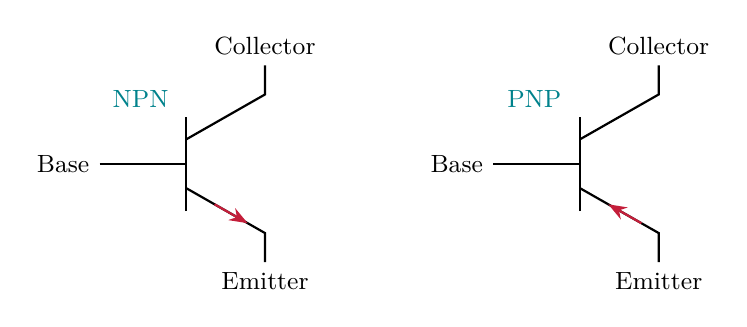
\begin{tikzpicture}[font=\small,line width=0.8pt]
\foreach \x/\name in {0/NPN,5.0/PNP}{
  \begin{scope}[shift={(\x,0)}]
  \draw (0,0)--(0,1.2) (-1.1,0.6)--(0,0.6);
  \draw (0,0.91)--(1.0,1.48)--(1.0,1.85);
  \draw (0,0.29)--(1.0,-0.28)--(1.0,-0.65);
  \node[left] at (-1.1,0.6) {Base};
  \node[above] at (1,1.85) {Collector};
  \node[below] at (1,-0.65) {Emitter};
  \node[myteal,above] at (-0.58,1.18) {\name};
  \end{scope}
}
\draw[-Stealth,myred,thick] (0.36,0.085)--(0.78,-0.155);
\draw[-Stealth,myred,thick] (5.78,-0.155)--(5.36,0.085);
\end{tikzpicture}
\end{tcolorbox}

\par\vspace{6pt}\noindent
\begin{tabularx}{\linewidth}{|B{3.3cm}|Y|Y|Y|}\hline
Region & \textbf{Emitter junction} & \textbf{Collector junction} & \textbf{Use or behaviour} \\ \hline
Cut-off & Reverse or effectively off & Reverse & Leakage only, switch open. \\ \hline
Forward active & Forward & Reverse & Current or voltage amplification. \\ \hline
Saturation & Forward & Forward & Switch on with small \(V_{CE}\). \\ \hline
Reverse active & Reverse & Forward & Roles are exchanged with reduced gain. \\ \hline
\end{tabularx}

For current magnitudes \(I_E=I_C+I_B\). Neglecting leakage in active operation,
\[
\begin{aligned}
\alpha&=\frac{I_C}{I_E},&
\beta&=\frac{I_C}{I_B},&
\gamma&=\frac{I_E}{I_B},\\
\beta&=\frac{I_C}{I_E-I_C}
      =\frac{\alpha}{1-\alpha},&
\alpha&=\frac{\beta}{1+\beta},&
\gamma&=1+\beta .
\end{aligned}
\]
\begin{itemize}[leftmargin=*, itemsep=3pt, topsep=4pt]
  \item \textbf{DC versus incremental gain.} DC ratios use the currents at one bias point. Incremental gains use small current changes around that point at fixed output voltage.
  \item \textbf{Check the operating mode.} Use \(I_C\approx\beta I_B\) in forward active operation. In saturation the external circuit mainly limits the collector current.
\end{itemize}

\subsection{CB, CE and CC characteristics}
\begin{itemize}[leftmargin=*, itemsep=3pt, topsep=4pt]
  \item \textbf{Common terminal.} This terminal belongs to both the input and output circuits.
  \item \textbf{Input characteristic.} Vary input voltage and record input current at a fixed output voltage.
  \item \textbf{Output characteristic.} Vary output voltage for a fixed input current. Repeat for different input currents. The table uses voltage magnitudes where convenient.
\end{itemize}
\par\vspace{6pt}\noindent
\begin{tabularx}{\linewidth}{|B{2cm}|Y|Y|Y|}\hline
Mode & \textbf{Input variables} & \textbf{Output variables} & \textbf{Gain and application} \\ \hline
CB & \(I_E,V_{BE}\) at fixed \(V_{CB}\). & \(I_C,V_{CB}\) at fixed \(I_E\). & Current gain \(\alpha<1\). Low input resistance. \\ \hline
CE & \(I_B,V_{BE}\) at fixed \(V_{CE}\). & \(I_C,V_{CE}\) at fixed \(I_B\). & Current gain \(\beta\). Resistively loaded voltage amplifier is inverting. \\ \hline
CC & \(I_B,V_{BC}\) at fixed \(V_{EC}\) for formal common-collector port variables. & \(I_E,V_{EC}\) at fixed \(I_B\). Voltage magnitudes may be plotted. & Current gain \(\gamma\). Emitter follower has nearly unity positive voltage gain and low output resistance. \\ \hline
\end{tabularx}

\begin{itemize}[leftmargin=*, itemsep=3pt, topsep=4pt]
  \item \textbf{Input curves.} CB and CE show a forward-junction shape in normal operation. In CC, \(V_{BE}=V_{BC}-V_{EC}\) relates the port voltage to the same junction.
  \item \textbf{CB and CC outputs.} In the active region \(I_C\approx\alpha I_E\) in CB and \(I_E\approx(1+\beta)I_B\) in CC. At fixed input current the output current changes only slightly with output voltage.
  \item \textbf{CE output.} Identify the low-voltage saturation knee, the active region with slight positive slope and the near-zero-base-current cut-off curve.
\end{itemize}

\begin{tcolorbox}[tikzbox,title={CE output characteristics and the Early effect},unbreakable]
\centering
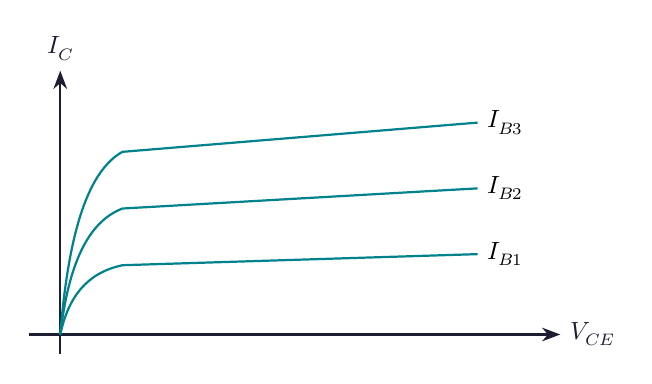
\begin{tikzpicture}[font=\small]
\draw[arrow] (-0.40,0)--(6.35,0) node[right] {$V_{CE}$};
\draw[arrow] (0,-0.25)--(0,3.35) node[above] {$I_C$};
\foreach \y/\lab in {0.88/1,1.60/2,2.32/3}{
  \draw[myteal,thick] (0,0) .. controls (0.10,{0.53*\y}) and (0.33,{0.89*\y})
  .. (0.79,\y) -- (5.3,{1.16*\y});
  \node[right] at (5.3,{1.16*\y}) {$I_{B\lab}$};
}
\end{tikzpicture}
\end{tcolorbox}

\begin{itemize}[leftmargin=*, itemsep=3pt, topsep=4pt]
  \item \textbf{Meaning.} The Early effect is modulation of the neutral base width.
  \item \textbf{Cause and effect.} Higher collector--base reverse bias narrows the neutral base, so collector current rises slightly in the active region.
  \item \textbf{Read the curve.} At fixed \(V_{BE}\), \(I_C\simeq I_{C0}(1+V_{CE}/V_A)\). Extend the active-region lines towards the voltage axis to estimate the intercept \(-V_A\). For \(V_A\gg V_{CE}\), the incremental output resistance is \(r_o\approx V_A/I_C\).
\end{itemize}

\subsection{Hybrid parameter model in outline}
The hybrid model is a linear two-port approximation for small signals near the DC bias (Q) point. It combines input resistance, reverse voltage ratio, forward current ratio and output admittance, giving it mixed units. For CE, use the port currents entering the device:
\[
\begin{aligned}
v_{be}&=h_{ie}i_b+h_{re}v_{ce},\\
i_c&=h_{fe}i_b+h_{oe}v_{ce}.
\end{aligned}
\]
\begin{itemize}[leftmargin=*, itemsep=3pt, topsep=4pt]
  \item \textbf{Set \(v_{ce}=0\).} Read input resistance \(h_{ie}=v_{be}/i_b\) in \(\Omega\) and forward current gain \(h_{fe}=i_c/i_b\) (dimensionless).
  \item \textbf{Set \(i_b=0\).} Read reverse voltage gain \(h_{re}=v_{be}/v_{ce}\) (dimensionless) and output admittance \(h_{oe}=i_c/v_{ce}\) in S.
  \item \textbf{Simplify the model.} The conditions above apply to small changes about the Q point. When \(h_{re}\) can be neglected, the output is a current source \(h_{fe}i_b\) in parallel with \(1/h_{oe}\).
\end{itemize}

\begin{tcolorbox}[examplebox,title={Convert BJT current gains}]
For a transistor in forward active mode with \(\alpha=0.98\) and \(I_E=2\,\mathrm{mA}\),
\[
\begin{aligned}
\beta&=\frac{0.98}{1-0.98}=49,\\
I_C&=0.98(2)=1.96\,\mathrm{mA},\\
I_B&=2-1.96=0.04\,\mathrm{mA}=40\,\mu\mathrm A.
\end{aligned}
\]
\end{tcolorbox}

\subsection{Junction field-effect transistor}
\begin{tcolorbox}[defbox,title={JFET and pinch-off}]
A junction field-effect transistor (JFET) is a voltage-controlled device in which a reverse-biased gate junction changes the width of a conducting channel. Pinch-off at the drain end marks the start of the nearly constant drain-current region. Cut-off is the gate-bias condition where channel current becomes negligible.
\end{tcolorbox}

\begin{itemize}[leftmargin=*, itemsep=3pt, topsep=4pt]
  \item \textbf{Bias and symbol.} Use \(V_{DS}>0\) and \(V_{GS}\le 0\) for an n-channel JFET. Its reverse-biased gate draws very little current. The gate arrow points into an n-channel and out of a p-channel.
  \item \textbf{Common-source circuit.} Ground the source, connect \(R_D\) from the drain to \(V_{DD}\), and set the gate bias separately.
  \item \textbf{Drain characteristics.} Vary \(V_{DS}\) at fixed \(V_{GS}\) and record \(I_D\). Repeat at different gate voltages to obtain a family of curves.
\end{itemize}

\begin{tcolorbox}[tikzbox,title={N-channel JFET in a common-source circuit},unbreakable]
\centering
\begin{tikzpicture}[font=\small]
\draw[thick] (2.6,0)--(2.6,1.71) (2.6,2.06)--(2.6,2.76)
 (2.6,3.43)--(2.6,3.89);
\draw[thick,line width=1.5pt] (2.6,1.05)--(2.6,2.06);
\draw[-Stealth,thick,myteal] (0.35,1.56)--(2.6,1.56);
\draw[thick] (2.46,2.76) rectangle (2.74,3.43);
\draw[thick] (2.28,0)--(2.92,0) (2.37,-0.10)--(2.83,-0.10) (2.47,-0.20)--(2.73,-0.20);
\node[left] at (0.35,1.56) {$V_{GS}\le0$};
\node[above] at (2.6,3.89) {$V_{DD}$};
\node[right] at (2.76,3.09) {$R_D$};
\node[right] at (2.76,2.16) {Drain};
\node[right] at (2.76,0.72) {Source};
\end{tikzpicture}
\end{tcolorbox}

At small \(V_{DS}\) the channel is nearly ohmic. Increasing \(V_{DS}\) widens its depletion region near the drain. Beyond the boundary \(V_{DS}\approx V_{GS}-V_P\), with \(V_P=V_{GS(\mathrm{off})}<0\), the drain current is nearly constant until breakdown. More negative gate voltage lowers the whole curve. The transfer characteristic in the saturation region is approximately
\[
I_D=I_{DSS}\left(1-\frac{V_{GS}}{V_P}\right)^2,\qquad V_P\le V_{GS}\le0 .
\]
Here \(I_{DSS}\) is the saturation drain current at \(V_{GS}=0\).

\begin{tcolorbox}[tikzbox,title={N-channel JFET transfer characteristic in saturation},unbreakable]
\centering
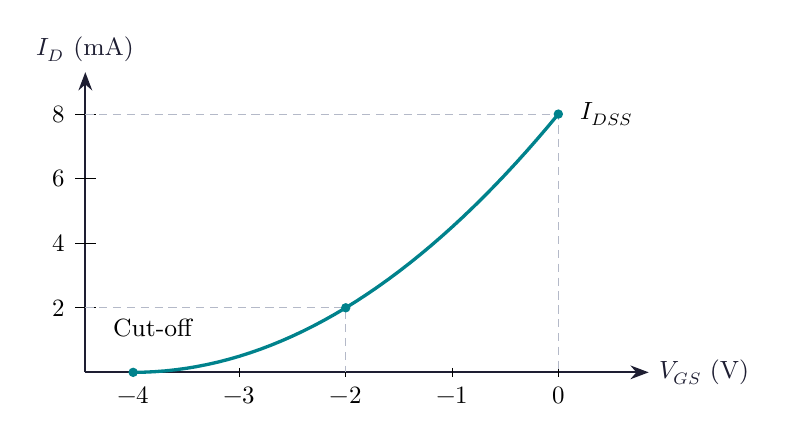
\begin{tikzpicture}[x=1.35cm,y=0.41cm,font=\small]
\draw[arrow] (-4.45,0)--(0.85,0) node[right] {$V_{GS}$ (V)};
\draw[arrow] (-4.45,0)--(-4.45,9.3) node[above] {$I_D$ (mA)};
\foreach \x in {-4,-3,-2,-1,0} {
  \draw (\x,0.14)--(\x,-0.14) node[below] {$\x$};
}
\foreach \y in {2,4,6,8} {
  \draw (-4.35,\y)--(-4.55,\y) node[left] {$\y$};
}
\draw[densely dashed,mgframe] (-4.45,2)--(-2,2)--(-2,0);
\draw[densely dashed,mgframe] (-4.45,8)--(0,8)--(0,0);
\draw[myteal,very thick,domain=-4:0,samples=41] plot (\x,{0.5*(\x+4)^2});
\fill[myteal] (-4,0) circle[radius=1.7pt]
             (-2,2) circle[radius=1.7pt]
             (0,8) circle[radius=1.7pt];
\node[anchor=west] at (-4.28,1.38) {Cut-off};
\node[anchor=west] at (0.12,8) {$I_{DSS}$};
\end{tikzpicture}
\end{tcolorbox}

\begin{tcolorbox}[examplebox,title={Read the gate-voltage curve and check the bias region}]
\begin{enumerate}[leftmargin=*, itemsep=3pt, topsep=4pt]
  \item \textbf{Read the endpoints.} At \(V_{GS}=0\), \(I_{DSS}=8\,\mathrm{mA}\). At \(V_{GS}=V_P=-4\,\mathrm V\), \(I_D\approx0\).
  \item \textbf{Read and check an intermediate point.} For \(V_{GS}=-2\,\mathrm V\), the curve gives \(2\,\mathrm{mA}\). The square-law model gives the same value:
  \[
    I_D=(8\,\mathrm{mA})\left(1-\frac{-2}{-4}\right)^2=2\,\mathrm{mA}.
  \]
  \item \textbf{Check \(V_{DS}\).} The knee of this drain curve is at \(V_{GS}-V_P=2\,\mathrm V\). Use the transfer-curve value at or above the knee and below breakdown. Below the knee, read the rising portion of the drain curve instead.
\end{enumerate}
\end{tcolorbox}

\subsection{MOSFET construction and output characteristics}
\begin{itemize}[leftmargin=*, itemsep=3pt, topsep=4pt]
  \item \textbf{Definition.} A metal--oxide--semiconductor field-effect transistor (MOSFET) uses an insulated gate to control the channel.
  \item \textbf{Construction.} An n-channel enhancement device has \(n^+\) source and drain regions in a p-type body. A thin insulator separates gate and body. Many discrete devices tie the body to the source.
  \item \textbf{Enhancement action.} Positive \(V_{GS}\) above the model threshold \(V_{TH}\) induces an inversion channel. A p-channel device uses opposite polarities and carrier types.
  \item \textbf{Depletion device.} It has a channel at \(V_{GS}=0\). Gate bias can reduce or increase channel conduction.
\end{itemize}

For a long-channel n-channel enhancement device with body tied to source, ignore subthreshold conduction and channel-length modulation. Define \(V_{\mathrm{ov}}=V_{GS}-V_{TH}\) and \(k_n=\mu_n C_{\mathrm{ox}}W/L\) in \(\mathrm{A/V^2}\). Then
\[
I_D=
\begin{cases}
0,& V_{GS}\le V_{TH},\\
k_n\bigl(V_{\mathrm{ov}}V_{DS}-V_{DS}^2/2\bigr),
   &0\le V_{DS}<V_{\mathrm{ov}},\\
k_n V_{\mathrm{ov}}^2/2,& V_{DS}\ge V_{\mathrm{ov}}>0 .
\end{cases}
\]
\begin{itemize}[leftmargin=*, itemsep=3pt, topsep=4pt]
  \item \textbf{Read the curve.} Each \(I_D\)--\(V_{DS}\) curve rises in the ohmic or triode region, reaches a knee at \(V_{DS}=V_{\mathrm{ov}}\) and flattens in saturation. A higher \(V_{GS}\) increases both the plateau current and knee voltage.
  \item \textbf{Choose the region.} Amplifiers normally bias a MOSFET in saturation. A fully enhanced switch operates in the low-resistance ohmic region. Real saturation curves slope upward slightly, and BJT saturation is a different bias condition.
\end{itemize}

\begin{tcolorbox}[tikzbox,title={FET drain characteristics (schematic)},unbreakable]
\centering
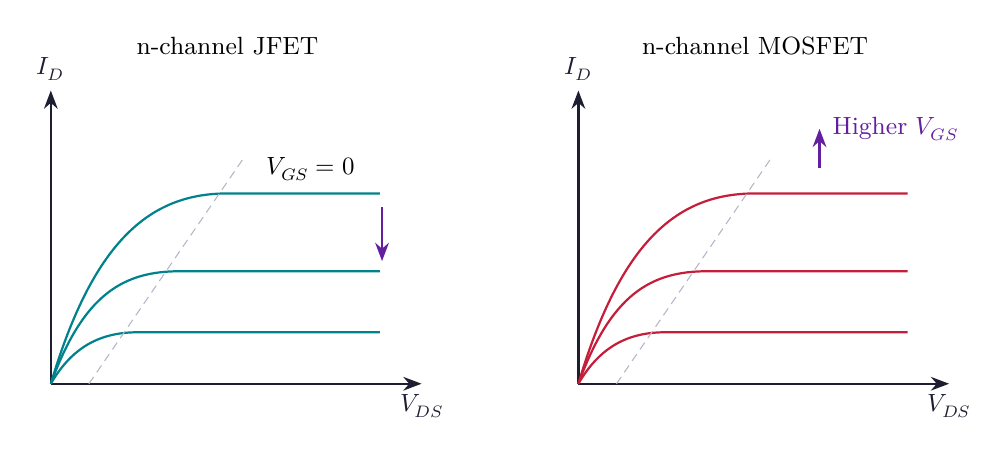
\begin{tikzpicture}[x=0.88cm,y=0.76cm,font=\small]
\begin{scope}
\draw[arrow] (0,0)--(5.35,0) node[below] {$V_{DS}$};
\draw[arrow] (0,0)--(0,4.90) node[above] {$I_D$};
\node[above] at (2.55,5.33) {n-channel JFET};
\draw[myteal,thick] (0,0) .. controls (0.62,2.42) and (1.45,3.18) .. (2.55,3.18)--(4.75,3.18);
\draw[myteal,thick] (0,0) .. controls (0.47,1.50) and (1.05,1.88) .. (1.86,1.88)--(4.75,1.88);
\draw[myteal,thick] (0,0) .. controls (0.30,0.60) and (0.70,0.86) .. (1.25,0.86)--(4.75,0.86);
\draw[densely dashed,mgframe] (0.55,0)--(2.80,3.80);
\node[above] at (3.75,3.22) {$V_{GS}=0$};
\draw[-Stealth,mypurple,thick] (4.78,2.95)--(4.78,2.05);
\end{scope}
\begin{scope}[xshift=6.7cm]
\draw[arrow] (0,0)--(5.35,0) node[below] {$V_{DS}$};
\draw[arrow] (0,0)--(0,4.90) node[above] {$I_D$};
\node[above] at (2.55,5.33) {n-channel MOSFET};
\draw[myred,thick] (0,0) .. controls (0.62,2.42) and (1.45,3.18) .. (2.55,3.18)--(4.75,3.18);
\draw[myred,thick] (0,0) .. controls (0.47,1.50) and (1.05,1.88) .. (1.86,1.88)--(4.75,1.88);
\draw[myred,thick] (0,0) .. controls (0.30,0.60) and (0.70,0.86) .. (1.25,0.86)--(4.75,0.86);
\draw[densely dashed,mgframe] (0.55,0)--(2.80,3.80);
\draw[-Stealth,mypurple,thick] (3.48,3.60)--(3.48,4.26) node[right=1pt] {Higher $V_{GS}$};
\end{scope}
\end{tikzpicture}
\par\smallskip\small
Dashed lines mark the transition into saturation. The JFET arrow points towards more negative \(V_{GS}\). The MOSFET shown is an enhancement device.
\end{tcolorbox}

\subsection{Op-amp model, open-loop response and parameters}
\begin{tcolorbox}[defbox,title={Operational amplifier}]
An op-amp is a high-gain differential voltage amplifier. It amplifies \(v_+-v_-\) and ideally rejects voltage common to both inputs. Negative feedback makes the closed-loop gain depend primarily on an external network.
\end{tcolorbox}

\begin{itemize}[leftmargin=*, itemsep=3pt, topsep=4pt]
  \item \textbf{Open-loop voltage response.} For small differential voltage, \(v_o=A_{\mathrm{OL}}(v_+-v_-)\). The steep transfer curve levels off at the positive and negative output swing limits.
  \item \textbf{Frequency response.} With a dominant pole, \(\lvert A_{\mathrm{OL}}\rvert\) is nearly flat at low frequency and falls at about \(20\,\mathrm{dB}\) per decade beyond the pole.
  \item \textbf{Ideal model.} Infinite open-loop gain, input resistance and bandwidth. Zero output resistance and offset. Perfect common-mode and supply rejection.
  \item \textbf{Use in circuit problems.} With stable negative feedback and linear operation, take \(i_+=i_-=0\) and \(v_+\approx v_-\). Check input range, output swing and slew rate before using these approximations.
\end{itemize}

\begin{itemize}[leftmargin=*, itemsep=3pt, topsep=4pt]
  \item \textbf{Input offset and bias.} Offset voltage is the differential voltage required for zero output. Bias current is the average of the input currents.
  \item \textbf{Gain-bandwidth product.} Approximately constant for a single dominant pole.
  \item \textbf{Slew rate.} Maximum output slope in V/\(\mu\)s. For a sinusoid with peak \(V_m\) and frequency \(f\), require \(\mathrm{SR}\ge 2\pi f V_m\), using consistent time units.
  \item \textbf{Rejection ratios.} \(\mathrm{CMRR}=20\log_{10}\lvert A_d/A_{\mathrm{cm}}\rvert\) in dB measures rejection of common-mode inputs. Supply rejection measures sensitivity to supply changes.
\end{itemize}

\subsection{Inverting, non-inverting, summing and difference amplifiers}
\begin{tcolorbox}[tikzbox,title={Inverting amplifier with negative feedback},unbreakable]
\centering
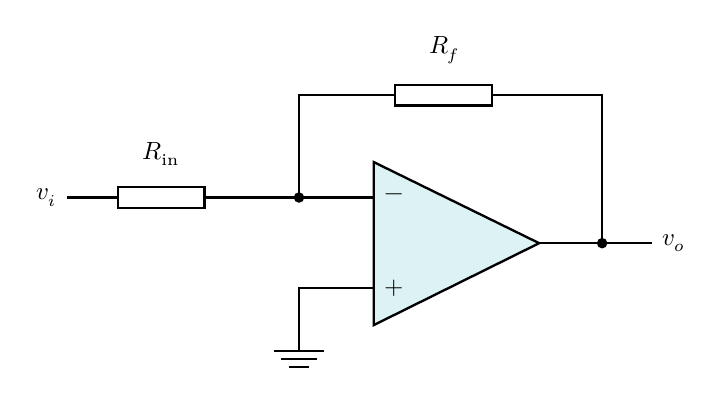
\begin{tikzpicture}[font=\small,line width=0.85pt]
\draw[fill=hdrteal] (4.25,0.08)--(4.25,2.15)--(6.35,1.12)--cycle;
\node at (4.51,1.70) {$-$};
\node at (4.51,0.55) {$+$};
\draw (0.36,1.70)--(1.0,1.70) (2.1,1.70)--(4.25,1.70);
\draw (1.0,1.57) rectangle (2.1,1.83);
\node[above=4pt] at (1.55,1.83) {$R_{\mathrm{in}}$};
\draw (3.30,1.70)--(3.30,3.00)--(4.52,3.00)
 (5.75,3.00)--(7.15,3.00)--(7.15,1.12);
\draw (4.52,2.87) rectangle (5.75,3.13);
\node[above=4pt] at (5.14,3.13) {$R_f$};
\draw (4.25,0.55)--(3.30,0.55)--(3.30,-0.25);
\draw (2.98,-0.25)--(3.62,-0.25) (3.07,-0.35)--(3.53,-0.35) (3.17,-0.45)--(3.43,-0.45);
\draw (6.35,1.12)--(7.78,1.12);
\fill (3.30,1.70) circle (1.9pt) (7.15,1.12) circle (1.9pt);
\node[left] at (0.36,1.70) {$v_i$};
\node[right] at (7.78,1.12) {$v_o$};
\end{tikzpicture}
\end{tcolorbox}

For the \textbf{inverting amplifier}, the non-inverting input is grounded. The inverting input is at virtual ground and draws negligible current. KCL at that node gives
\[
\begin{aligned}
\frac{v_i-0}{R_{\mathrm{in}}}&=\frac{0-v_o}{R_f},\\
v_o&=-\frac{R_f}{R_{\mathrm{in}}}v_i.
\end{aligned}
\]
For the \textbf{non-inverting amplifier}, \(v_+=v_i\). Connect \(R_g\) from the inverting node to ground and \(R_f\) from output to that node:
\[
\begin{aligned}
v_-&=\frac{R_g}{R_g+R_f}v_o,\\
v_o&=\left(1+\frac{R_f}{R_g}\right)v_i .
\end{aligned}
\]
Direct negative feedback gives a unity-gain voltage follower with high input resistance and low output resistance.

For an \textbf{inverting summer}, several voltages \(v_k\) feed the virtual-earth node through separate resistors \(R_k\). KCL adds the currents, giving \(v_o=-R_f\sum_k v_k/R_k\). With equal input resistors the circuit gives a scaled sum.

For a \textbf{difference amplifier}, connect \(v_1\) through \(R_1\) to the inverting node, \(R_2\) from output to that node, \(v_2\) through \(R_3\) to the non-inverting node and \(R_4\) from that node to ground. Then
\[
\begin{aligned}
v_+ &= \frac{R_4}{R_3+R_4}v_2,\\
\frac{v_1-v_+}{R_1}&=\frac{v_+-v_o}{R_2},\\
v_o&=\left(1+\frac{R_2}{R_1}\right)
      \frac{R_4}{R_3+R_4}v_2-\frac{R_2}{R_1}v_1.
\end{aligned}
\]
When \(R_2/R_1=R_4/R_3=k\), this reduces to \(v_o=k(v_2-v_1)\). Resistor-ratio mismatch gives some common-mode gain.

\begin{tcolorbox}[examplebox,title={Closed-loop gain and output swing}]
An inverting amplifier has \(R_{\mathrm{in}}=10\,\mathrm{k}\Omega\), \(R_f=47\,\mathrm{k}\Omega\), and practical output limits of \(\pm 10\,\mathrm V\).
\[
\begin{aligned}
A_v&=-\frac{47}{10}=-4.7,\\
v_o&=(-4.7)(0.8)=-3.76\,\mathrm V .
\end{aligned}
\]
A \(3\,\mathrm V\) input would require \(-14.1\,\mathrm V\), so the output instead clips near the negative limit and the virtual-ground relation no longer applies. For the matched difference-amplifier ratios \(k=4.7\), \(v_1=0.4\,\mathrm V\) and \(v_2=0.8\,\mathrm V\), the linear output is \(4.7(0.8-0.4)=1.88\,\mathrm V\).
\end{tcolorbox}

\newpage
\begin{center}
  {\large\bfseries\color{myred} Quick Revision --- Module 6}\\[3pt]
  {\small\color{mydark} Transistors and Operational Amplifiers $|$ 26-ES-EE101}
\end{center}
\noindent{\color{myred}\rule{\linewidth}{1.2pt}}
\vspace{4pt}

\begin{tcolorbox}[formulabox, title={Key Formulas and Concepts at a Glance}]
\renewcommand{\arraystretch}{1.35}
\begin{tabularx}{\linewidth}{B{4.4cm}Y}
BJT current ratios & $\beta=\alpha/(1-\alpha)$; $\gamma=1+\beta$. \\[3pt]
JFET saturation current & $I_D=I_{DSS}(1-V_{GS}/V_P)^2$ in its valid bias range. \\[3pt]
Op-amp voltage gains & $-R_f/R_{\mathrm{in}}$ (inverting); $1+R_f/R_g$ (non-inverting). \\[3pt]
Matched difference amplifier & $v_o=(R_2/R_1)(v_2-v_1)$. \\[3pt]
Inverting summer & $v_o=-R_f\sum_k v_k/R_k$. \\[3pt]
\end{tabularx}
\end{tcolorbox}

\begin{tcolorbox}[defbox, title={One-Line Definitions}]
\textbf{Early effect.} Change of collector current with collector voltage due to modulation of the neutral base width.

\textbf{Transconductance.} Incremental change in output current per unit input voltage.

\textbf{Virtual short.} Nearly equal op-amp input voltages under linear negative feedback.

\textbf{Slew rate.} Maximum rate at which an amplifier output voltage can change.
\end{tcolorbox}

\begin{tcolorbox}[exambox, title={Frequently Asked / Viva Questions}]
\begin{enumerate}[topsep=0pt, label=\textbf{Q\arabic*.}, itemsep=5pt]
  \item \Q{Why is the BJT base thin?} Most injected carriers cross it before recombining.
  \item \Q{Which junctions are forward biased in BJT saturation?} Both emitter--base and collector--base junctions.
  \item \Q{What gain does the common-collector connection give?} It gives current gain $\gamma=1+\beta$ and approximately unity voltage gain.
  \item \Q{What causes the slope of CE active characteristics?} The Early effect from base-width modulation.
  \item \Q{Why are h-parameters called hybrid?} Their units include ohms, siemens and dimensionless ratios.
  \item \Q{Does JFET pinch-off mean zero drain current?} Pinch-off starts current saturation. Gate cut-off is the near-zero-current condition.
  \item \Q{What forms the enhancement MOSFET channel?} Gate bias above threshold induces a conducting inversion layer.
  \item \Q{When can we equate the op-amp input voltages?} With high gain, stable negative feedback and linear operation.
  \item \Q{What determines an inverting amplifier gain?} The resistor ratio $-R_f/R_{\mathrm{in}}$.
  \item \Q{When does a difference amplifier reject common-mode input?} When the resistor ratios match and the op-amp is within its linear limits.
  \item \Q{What does slew rate limit?} Maximum output slope and therefore large-signal response at high frequency.
\end{enumerate}
\end{tcolorbox}

\begin{tcolorbox}[tikzbox, title={Summary Reference}]
\begin{tabularx}{\linewidth}{|B{4.0cm}|Y|}\hline
Topic & \textbf{What to remember} \\ \hline
BJT & Base controls collector current. Check active or saturated bias. \\ \hline
JFET and MOSFET & A reverse-biased junction or insulated gate controls a conducting channel. \\ \hline
Op-amp & Show the feedback connection, apply KCL, then test the output swing. \\ \hline
\end{tabularx}
\end{tcolorbox}

\end{document}

